\section{Struktur Kepang}\label{sec:braiding}
Operasi $\otimes$ dalam kategori monoidal umumnya tidak disyaratkan komutatif. Namun, dalam banyak contoh, fenomena komutativitas tidak hanya hadir tetapi juga sangat penting. Tujuan struktur kepang ialah menjelaskan komutativitas operasi $\otimes $. Seperti pada objek satuan dan hukum asosiatif, yang diperlukan di sini adalah suatu keluarga isomorfisme, bukan kesamaan ketat; keluarga ini juga disebut \emph{kendala komutativitas}. Asal penamaan struktur kepang akan dijelaskan dalam Contoh \ref{eg:braid}. Salah satu sumber awalnya adalah \cite{JS93}.

\begin{definition}\label{def:braiding}\index{bianjiegou@struktur kepang (braiding)}\index{liujiaoxinggongli@aksioma segienam (hexagon axiom)}
	Misalkan $(\mathcal{V}, \otimes, a, \munit, \iota)$ kategori monoidal. Suatu \emph{struktur kepang} pada kategori ini berarti isomorfisme antara fungtor biner
	\[ c(X,Y): X \otimes Y \rightiso Y \otimes X, \quad X, Y \in \Obj(\mathcal{V}) \]
	(yakni, natural terhadap peubah $X, Y$), sedemikian sehingga diagram-diagram berikut komutatif:
	\begin{equation}\label{eqn:hexagon-axiom-1}\begin{tikzcd}[row sep=small]
		{} & X \otimes (Y \otimes Z) \arrow[r, "{c(X, Y \otimes Z)}" inner sep=1em] & (Y \otimes Z) \otimes X \arrow[rd] & \\
		(X \otimes Y) \otimes Z \arrow[ru] \arrow[rd, "{c(X,Y) \otimes \identity}"'] & & & Y \otimes (Z \otimes X) \\
		& (Y \otimes X) \otimes Z \arrow[r] & Y \otimes (X \otimes Z) \arrow[ru, "{\identity \otimes c(X,Z)}"'] &
	\end{tikzcd}\end{equation}
	\begin{equation}\label{eqn:hexagon-axiom-2}\begin{tikzcd}[row sep=small]
		{} & (X \otimes Y) \otimes Z \arrow[r, "{c(X \otimes Y, Z)}" inner sep=1em] & Z \otimes (X \otimes Y) \arrow[rd] & \\
		X \otimes (Y \otimes Z) \arrow[ru] \arrow[rd, "{\identity \otimes c(Y, Z)}"'] & & & (Z \otimes X) \otimes Y \\
		& X \otimes (Z \otimes Y) \arrow[r] & (X \otimes Z) \otimes Y \arrow[ru, "{c(X, Z) \otimes \identity}"'] &
	\end{tikzcd}\end{equation}
	serta
	\begin{equation}\begin{tikzcd}
		\munit \otimes X \arrow[rd, "\lambda_X"'] \arrow[rr, "{c(\munit, X)}"] & & X \otimes \munit \arrow[ld, "\rho_X"] \\
		& X &
	\end{tikzcd} \quad \begin{tikzcd}
		X \otimes \munit \arrow[rd, "\rho_X"'] \arrow[rr, "{c(X, \munit)}"] & & \munit  \otimes X \arrow[ld, "\lambda_X"] \\
		& X &
	\end{tikzcd}\end{equation}
	dengan $X,Y,Z$ sebarang objek dalam $\mathcal{V}$; semua panah tanpa label adalah kendala asosiativitas atau inversnya.
\end{definition}

Kategori monoidal yang dilengkapi struktur kepang $c$ singkatnya disebut kategori monoidal berkepang. Diagram \eqref{eqn:hexagon-axiom-1} dan \eqref{eqn:hexagon-axiom-2} umumnya disebut aksioma segienam.
\begin{remark}\label{rem:hexagon-axiom-strict}
	Untuk kategori monoidal ketat (Definisi \ref{def:strict-monoidal-cat}), aksioma segienam dapat ditulis sebagai
	\begin{align*}
		c(X \otimes Y, Z) & = (c(X, Z) \otimes \identity_Y) (\identity_X \otimes c(Y, Z)), \\
		c(X, Y \otimes Z) & = (\identity_Y \otimes c(X, Z)) (c(X, Y) \otimes \identity_Z)
	\end{align*}
\end{remark}

\begin{definition}\index{yaobanhanzi@fungtor monoidal (monoidal functor)!berkepang (braided)}
	Misalkan $\mathcal{V}_1, \mathcal{V}_2$ kategori monoidal. Fungtor monoidal $F: \mathcal{V}_1 \to \mathcal{V}_2$ disebut fungtor monoidal berkepang jika memenuhi sifat berikut: untuk sebarang objek $X, Y$, diagram berikut komutatif.
	\[ \begin{tikzcd}[column sep=small]
		FX \otimes FY \arrow[r] \arrow[d, "{c_2(FX, FY)}"'] & F(X \otimes Y) \arrow[d, "{Fc_1(X, Y)}"] \\
		FY \otimes FX \arrow[r] & F(Y \otimes X)
	\end{tikzcd} \]
\end{definition}

\begin{definition}\label{def:symm-monoidal-cat}\index{yaobanfanchou@kategori monoidal (monoidal category)!kategori monoidal simetris (symmetric monoidal category)}
	Misalkan $(\mathcal{V}, \otimes, a, \munit, \iota, c)$ kategori monoidal berkepang. Jika syarat simetri $c(Y,X) \circ c(X, Y) = \identity_{X \otimes Y}$ berlaku untuk semua $X, Y$, kategori tersebut disebut \emph{kategori monoidal simetris}.
\end{definition}

\begin{example}
	Kategori-kategori monoidal yang dibangun dari produk dan koproduk dalam Contoh \ref{eg:monoidal-cat} semuanya mempunyai struktur kepang yang natural (lihat Lema \ref{prop:product-commutativity}). Demikian pula, kategori modul atas gelanggang komutatif $R$, yakni $R\dcate{Mod}$, mempunyai struktur kepang natural sebagai berikut:
	\begin{align*}
		c(M, N): M \dotimes{R} N & \longrightarrow N \dotimes{R} M \\
		m \otimes n & \longmapsto n \otimes m, \quad m \in M, n \in N.
	\end{align*}
	Semua kategori monoidal berkepang ini bersifat simetris. Perinciannya dapat dilihat dalam \S\ref{sec:module-tensor-prod}.
\end{example}

\begin{proposition}[Persamaan Yang--Baxter]\label{prop:YBE-cat-strict}\index{YBE@persamaan Yang--Baxter (Yang--Baxter equation)}
	Misalkan $\mathcal{V}$ kategori monoidal berkepang. Bagian yang digambar dengan garis utuh pada diagram berikut komutatif untuk sebarang objek $X, Y, Z$.
	\begin{center}\small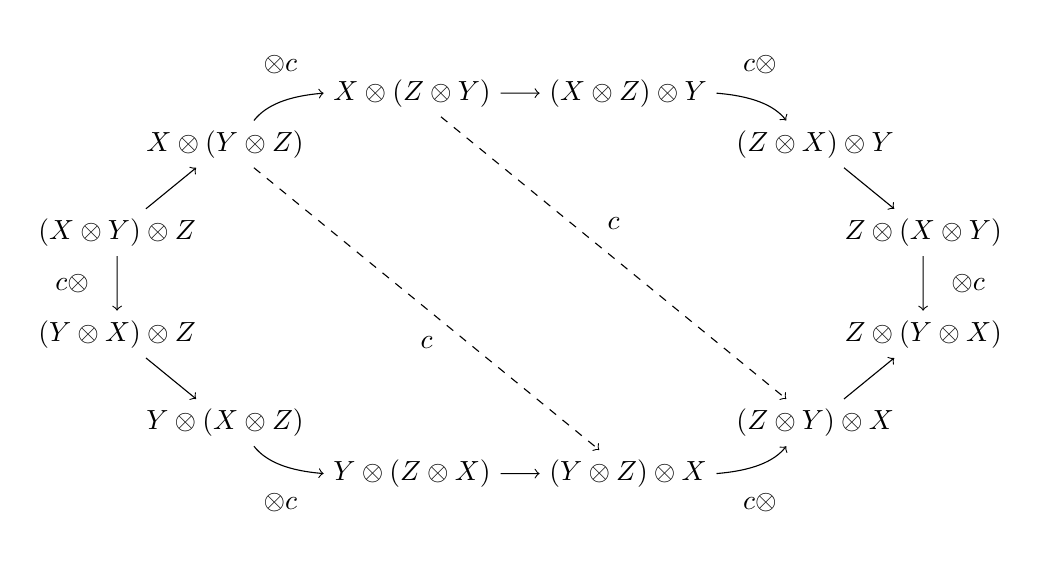
\begin{tikzpicture}[xscale=5.3, yscale=2.5, every edge/.style={draw, ->}, C/.style={inner sep=1em}]
		\node (A1) at (75:1cm) {$(X \otimes Z) \otimes Y$};
		\node (A2) at (105:1cm) {$X \otimes (Z \otimes Y)$};
		\node (A3) at (135:1cm) {$X \otimes (Y \otimes Z)$};
		\node (A4) at (165:1cm) {$(X \otimes Y) \otimes Z$};
		\node (A5) at (195:1cm) {$(Y \otimes X) \otimes Z$};
		\node (A6) at (225:1cm) {$Y \otimes (X \otimes Z)$};
		\node (A7) at (255:1cm) {$Y \otimes (Z \otimes X)$};
		\node (A8) at (285:1cm) {$(Y \otimes Z) \otimes X$};
		\node (A9) at (315:1cm) {$(Z \otimes Y) \otimes X$};
		\node (A10) at (345:1cm) {$Z \otimes (Y \otimes X)$};
		\node (A11) at (15:1cm) {$Z \otimes (X \otimes Y)$};
		\node (A12) at (45:1cm) {$(Z \otimes X) \otimes Y$};

		\draw (A4) edge (A3);	\draw (A3) edge[bend left] node[C, above] {$\identity \otimes c$} (A2); \draw (A2) edge (A1); \draw (A1) edge[bend left] node[C, above] {$c \otimes \identity$} (A12); \draw (A12) edge (A11); \draw (A11) edge node[C, right] {$\identity \otimes c$} (A10);

		\draw (A4) edge node[C, left] {$c \otimes \identity$} (A5); \draw (A5) edge (A6); \draw (A6) edge[bend right] node[C, below] {$\identity \otimes c$} (A7); \draw (A7) edge (A8); \draw (A8) edge[bend right] node[C, below] {$c \otimes \identity$} (A9); \draw (A9) edge (A10);
	
		\draw[dashed] (A3) edge node[C, below] {$c$} (A8);
		\draw[dashed] (A2) edge node[C, above] {$c$} (A9);
	\end{tikzpicture}\end{center}
	Di sini semua panah tanpa label adalah kendala asosiativitas, sedangkan $c$ menyatakan kendala komutativitas yang jelas dari konteks.
\end{proposition}
\begin{proof}
	Garis-garis putus-putus membagi diagram besar menjadi tiga bagian. Bagian kiri dan kanan komutatif karena aksioma segienam. Segi empat di tengah komutatif karena naturalitas $c$. Jadi, seluruh diagram komutatif.
\end{proof}

\begin{remark}\label{rem:YBE-cat-strict}
	Jika $\mathcal{V}$ kategori monoidal ketat, diagram di atas menyusut menjadi enam suku dan komutativitasnya tidak lain menyatakan
	\begin{multline*}
		(c(Y,Z) \otimes \identity_X) \, (\identity_Y \otimes c(X, Z)) \, (c(X, Y) \otimes \identity_Z) = \\
		(\identity_Z \otimes c(X, Y)) \, (c(X, Z) \otimes \identity_Y) \, (\identity_X \otimes c(Y, Z)).
	\end{multline*}
	Jika $\mathcal{V}$ adalah kategori ruang vektor yang membentuk kategori monoidal berkepang terhadap hasil kali tensor dan $X=Y=Z$, kesamaan di atas berkaitan dengan persamaan Yang--Baxter dalam fisika statistik (``Yang'' merujuk kepada Chen-Ning Yang). Penjelasan lebih lanjut akan diberikan dalam latihan.
\end{remark}

\begin{example}\label{eg:braid}\index[sym1]{Braid@$\cate{Braid}$}
	Berikut ini kita membangun kategori kepang \cate{Braid} dari sudut pandang topologis. Misalkan $n \in \Z_{\geq 1}$ dan definisikan
	\[ C_n := \left\{ \text{subhimpunan}\; c \subset \R^2: |c|=n \right\}, \]
	atau, dengan kata lain, ruang hasil bagi $\left\{ (y_1, \ldots, y_n) \in (\R^2)^n: \text{unsur-unsurnya berbeda} \right\}$ oleh aksi grup permutasi; ruang ini secara natural dilengkapi suatu topologi. Mulai sekarang, tetapkan $p = \{p_1, \ldots, p_n\} \in C_n$. Sebuah kepang dengan $n$ untai didefinisikan sebagai peta kontinu $x: [0,1] \to C_n$ yang memenuhi $x(0) = x(1) = p$. Secara visual, jika waktu $t$ dijadikan sumbu vertikal, lintasan $x$ memberikan $n$ kurva kontinu dalam $\R^3$ yang masing-masing tidak berpotongan dengan dirinya sendiri dan saling tidak berpotongan, serta bergerak naik dari $\{(p_1, 0), \ldots, (p_n, 0) \}$ ke $\{ (p_1, 1), \ldots, (p_n, 1) \}$; inilah yang disebut kepang. Jika kepang $x_1$ dapat dideformasi secara kontinu menjadi $x_2$ dengan titik-titik ujung $p$ tetap sepanjang deformasi, maka $x_1$ dan $x_2$ disebut ekuivalen. Selanjutnya, istilah kepang selalu berarti kelas ekuivalensi. Himpunan semua kepang dengan $n$ untai dinotasikan dengan $\mathcal{B}_n$.

	Meskipun kepang dapat dipandang sebagai gambar dalam $\R^3$, kita lazim meratakannya pada suatu bidang $L \simeq \R^2$. Proses ini dapat membuat proyeksi kurva-kurva tersebut berpotongan, tetapi dengan perturbasi kecil pada $L$ dapat dipastikan bahwa proyeksi tiga kurva tidak pernah bertemu pada satu titik. Tanpa mengurangi keumuman, dapat pula diasumsikan bahwa ujung-ujung bawah dan atas kepang masing-masing dipetakan ke $(i, 0), (i, 1) \in \R^2$, dengan $i=1, \ldots, n$. Untuk mempertahankan informasi ruangnya, pada setiap titik potong proyeksi dua kurva kita tandai kurva mana yang melintas di atas dan mana yang di bawah. Sebagai contoh, perhatikan kasus $n=3$:
	\begin{center}\begin{tikzpicture}[baseline=(braid), yscale=0.75]
		\braid[style strands={1}, style strands={2}, style strands={3}] (braid) s_1 s_2^{-1};
		\node[left=1em] (A) at (braid-1-s) {$t=1$};
		\node[left=1em] (B) at (braid-2-e) {$t=0$};
		\draw[-Latex, ultra thick] (B) -- (A);
		\node[below] at (braid-1-e) {$3$};
		\node[below] at (braid-2-e) {$1$};
		\node[below] at (braid-3-e) {$2$};
	\end{tikzpicture} \quad dan \quad \begin{tikzpicture}[baseline=(braid), yscale=0.75]
		\braid[style strands={1}, style strands={2}, style strands={3}] (braid)  s_2 s_1^{-1};
		\node[below] at (braid-1-e) {$2$};
		\node[below] at (braid-2-e) {$3$};
		\node[below] at (braid-3-e) {$1$};
	\end{tikzpicture}\end{center}

	Untuk sebarang $x, y \in \mathcal{B}_n$, definisikan komposisi $xy$ dengan menyambungkan peta $x,y: [0,1] \to C_n$ dari ujung ke ujung; secara visual, ini berarti merekatkan ujung awal $x$ pada ujung akhir $y$ untuk memperoleh kepang baru. Mudah dilihat bahwa operasi ini terdefinisi dengan baik. Sebagai contoh, jika kedua kepang di atas berturut-turut dinotasikan dengan $x,y$, maka
	\[ xy \; = \;
		\begin{array}{|c|c|} \hline x \\ \hline y \\ \hline \end{array} \quad = \quad
		\begin{tikzpicture}[yscale=0.75, baseline=(braid)]
		\braid[style strands={1}, style strands={2}, style strands={3},
			floor command={
			\draw[dashed] (\floorsx,\floorsy) -- (\floorex,\floorsy);
			}] (braid)
		s_1 s_2^{-1} | s_2 s_1^{-1};
	\end{tikzpicture}\]
	Dengan meluruskan setiap untai pada gambar di atas, terlihat bahwa kepang tersebut ekuivalen dengan tiga untai vertikal $\vert\;\vert\;\vert$. Dari sudut pandang aljabar, $\mathcal{B}_n$ bersama operasi komposisi kepang membentuk grup yang disebut \emph{grup kepang Artin}. Asosiativitas perkalian sudah jelas, sedangkan unsur satuannya adalah $\underbracket{\vert \cdots \vert}_{n \text{untai}}$, atau, dengan kata lain, fungsi konstan $[0,1] \to \{p\} \subset C_n$. Invers suatu kepang $x$ diperoleh dengan menelusuri kurva $x: [0,1] \to C_n$ dalam arah sebaliknya, atau, setelah diratakan pada bidang $\R^2$, dengan mengambil cerminan vertikalnya. Pembaca yang mengenal topologi akan segera melihat bahwa $\mathcal{B}_n = \pi_1(C_n, p)$; lihat Contoh \ref{eg:fundamental-groupoid}.

	Dengan konvensi, $\mathcal{B}_0$ adalah grup trivial. Dalam \S\ref{sec:symmetric-group}, kita akan menyelidiki beberapa sifat $\mathcal{B}_n$ dari sudut pandang teori grup serta hubungannya dengan grup simetris $\mathfrak{S}_n$; suatu presentasi grup $\mathcal{B}_n$ akan diberikan dalam \eqref{eqn:braid-presentation}.\index{bianqun@grup kepang (braid group)}\index[sym1]{B_n@$\mathcal{B}_n$}

	Sekarang kita bangun kategori monoidal ketat $\cate{Braid}$: himpunan objeknya adalah $\Z_{\geq 0}$, sedangkan himpunan morfisme antara sebarang dua objek $n,m$ didefinisikan sebagai $\mathcal{B}_n$ jika $n=m$, dan sebagai himpunan kosong jika tidak. Komposisi morfisme adalah komposisi dalam grup kepang. Selanjutnya, definisikan $m \otimes n := m+n$; untuk $x \in \mathcal{B}_m$, $y \in \mathcal{B}_n$, morfisme $x \otimes y \in \mathcal{B}_{m+n}$ didefinisikan dengan menempatkan kedua kepang berdampingan, yang secara visual dinyatakan sebagai
	\begin{center} 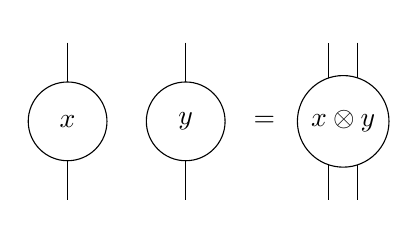
\begin{tikzpicture}[baseline=(current bounding box.center),
		 midbraid/.style={midway, draw, fill=white, shape=circle, minimum size=1cm} ]
		\draw (0,1) -- (0,-1) node[midbraid] {$x$};
		\draw (1.5,1) -- (1.5,-1) node[midbraid] {$y$};
		\node at (2.5,0) {$=$};
		\draw[double distance=10pt] (3.5, 1) -- (3.5,-1) node[midbraid] {$x \otimes y$};
	\end{tikzpicture}\end{center}
	Jelas bahwa $x \otimes y$ terdefinisi dengan baik, dan operasi ini menjadikan $\cate{Braid}$ kategori monoidal ketat; objek satuannya adalah $0$.

	Sekarang definisikan kendala komutativitas $c$ untuk memperoleh kategori monoidal berkepang. Untuk $X=m$, $Y=n$, kita menggunakan
	
\begin{tikzpicture} \draw[black, line width=3pt] (0,0) -- (0.5, 0); \end{tikzpicture}
	untuk menyatakan $m$ untai tak terjalin yang bersesuaian dengan objek $X$, sedangkan
	
\begin{tikzpicture} \draw[lightgray, line width=3pt] (0,0) -- (0.5, 0); \end{tikzpicture}
	menyatakan $n$ untai tak terjalin yang bersesuaian dengan objek $Y$. Definisikan $c(X, Y) \in \mathcal{B}_{m+n}$ sebagai
	\[ c(m,n) \;= \; \begin{tikzpicture}[baseline=(braid)]
		\braid[style strands={1}{lightgray}, style strands={2}{black}, line width=3pt] (braid) s_1;
		\node[above] at (braid-1-s) {$n$};
		\node[above] at (braid-2-s) {$m$};
		\node[below] at (braid-1-e) {$n$};
		\node[below] at (braid-2-e) {$m$};
	\end{tikzpicture}\]
	Ini berarti bahwa $n$ untai 
\begin{tikzpicture} \draw[lightgray, line width=3pt] (0,0)--(0.5,0); \end{tikzpicture} dipandang sebagai satu kesatuan dan dilintaskan di atas $m$ untai yang dinyatakan oleh 
\begin{tikzpicture} \draw[black, line width=3pt] (0,0)--(0.5,0); \end{tikzpicture}. Jika $X$ atau $Y$ selanjutnya dibagi menjadi dua kelompok $U, V$ dan diagram kepang yang bersesuaian digambar (berbentuk
	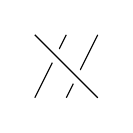
\begin{tikzpicture}[baseline=(current bounding box.center), scale=0.4, wline/.style={color=white, line width=1.8mm}]
		\draw (1,2) -- (0,0);
		\draw (2,2) -- (1,0);
		\draw[wline] (0,2) -- (2,0); \draw (0,2) -- (2,0);
	\end{tikzpicture}
	atau
	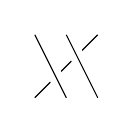
\begin{tikzpicture}[baseline=(current bounding box.center), scale=0.4, wline/.style={color=white, line width=1.8mm}]
		\draw (2,2) -- (0,0);
		\draw[wline] (0,2) -- (1,0); \draw (0,2) -- (1,0);
		\draw[wline] (1,2) -- (2,0); \draw (1,2) -- (2,0);
	\end{tikzpicture} ),
	aksioma segienam dapat diverifikasi (Catatan \ref{rem:hexagon-axiom-strict}); perinciannya diserahkan kepada pembaca.

	Persamaan Yang--Baxter (Catatan \ref{rem:YBE-cat-strict}) dapat diterjemahkan menjadi kesamaan yang langsung terlihat:
	\[ \begin{tikzpicture}[yscale=0.6, baseline=(braid)]
		\braid[style strands={1}, style strands={2}, style strands={3}] (braid) s_1 s_2 s_1;
	\end{tikzpicture}
	\qquad = \qquad
	\begin{tikzpicture}[yscale=0.6, baseline=(braid)]
		\braid[style strands={1}, style strands={2}, style strands={3}] (braid) s_2 s_1 s_2;
	\end{tikzpicture} \]

	Dengan cara yang sama, naturalitas kendala komutativitas dapat ditafsirkan secara intuitif sebagai berikut.
	\begin{center}
	$\begin{tikzcd}
		X \otimes Y \arrow[d, "{f \otimes g}"'] \arrow[r, "{c(X, Y)}"] & Y \otimes X \arrow[d, "{g \otimes f}"] \\
		X' \otimes Y' \arrow[r, "{c(X', Y')}"'] & Y' \otimes X'
	\end{tikzcd}$ \quad komutatif ekuivalen dengan \quad
	\begin{tikzpicture}[baseline=(braid),
		midbraid/.style={shape=circle, draw, fill=white, thick, outer sep=0pt, inner sep=0pt, minimum size=5mm} ]
		\coordinate (B1) at (0, 0);
		\coordinate (B2) at (2.2, 0);
		\braid[style strands={1}{lightgray}, style strands={2}{black}, line width=3pt] (bone) at (B1) s_1;
		\node at (bone-1-s) [midbraid, below=3pt] {\small $g$};
		\node at (bone-2-s) [midbraid, below=3pt] {\small $f$};
		\braid[style strands={1}{lightgray}, style strands={2}{black}, line width=3pt] (btwo) at (B2) s_1;
		\node at (btwo-1-e) [midbraid, above=3pt] {\small $g$};
		\node at (btwo-2-e) [midbraid, above=3pt] {\small $f$};
		\node at ($(bone.center)!.5!(btwo.center)$) {$=$};
	\end{tikzpicture}\end{center}
	Karena
	\begin{tikzpicture}[baseline=(braid), scale=0.5]
		\braid[style strands={1}{black}, style strands={2}{black}] (braid) s_1;
	\end{tikzpicture} $\neq$
	\begin{tikzpicture}[baseline=(braid), scale=0.5]
		\braid[style strands={1}{black}, style strands={2}{black}] (braid) s_1^{-1};
	\end{tikzpicture},
	kategori monoidal $\cate{Braid}$ tidak simetris; sesungguhnya, $c(1, 1)$ membangkitkan grup siklik tak hingga $\mathcal{B}_2 \simeq \Z$, sebagaimana tampak secara intuitif.
\end{example}

Kita telah mengandalkan intuisi topologis untuk memverifikasi semua sifat struktur kepang pada $\cate{Braid}$. Sebaliknya, dapat dibuktikan bahwa segala relasi yang dipenuhi morfisme-morfisme dalam $\cate{Braid}$ terhadap komposisi, yakni berbagai kesamaan diagram kepang, sudah mencakup semua sifat umum kategori monoidal berkepang \cite[Corollary 2.6]{JS93}; dalam ``jargon'' matematikawan, $\cate{Braid}$ adalah ``kategori monoidal berkepang bebas yang dibangkitkan oleh objek $1$''. Dengan kata lain, sifat umum kategori monoidal berkepang dapat diperiksa secara intuitif dalam $\cate{Braid}$. Dibandingkan dengan aksioma-aksioma pada Definisi \ref{def:braiding}, kesamaan antardiagram kepang sering kali langsung terlihat; pembaca kiranya telah menyaksikannya dengan jelas dalam pembahasan persamaan Yang--Baxter.

